\documentclass[a4paper]{article}

\usepackage{INTERSPEECH2021}

% Put the lab number of the corresponding exercise
\title{NLU course projects lab 6: SA}
\name{Nicola Muraro (248449)}

\address{
  University of Trento}
\email{nicola.muraro@studenti.unitn.it}

\begin{document}

\maketitle

\section{Introduction}
This last assignment is about the task of aspect-based sentiment analysis.
In this type of task, we generally aim to identify the polarity that each token has within the sentence. However, in our case, we focused on a slightly simpler task: the extraction of terms within the sentence, ignoring the part involving the prediction of their polarity.
To achieve this, we once again started by using a pre-trained language model. We used BERT also in this case. We then performed fine-tuning of this model to align the architecture’s predictions with our specific use case.

\section{Implementation details}
The type of architecture used for this assignment is comparable to the one I previously developed for the slot filling and intent classification tasks.
Here as well, we used BERT as the foundation to obtain a latent representation, which is subsequently passed through a dropout layer and finally processed by a fully connected layer to predict the type of term. The fine-tuning was performed on this entire structure, using the Laptop partition of the SemEval2014 Task 4 dataset.

Consequently, as a starting point for this implementation, I used the code developed in the previous assignment, making some modifications to adapt it to this specific task.
Additionally, my implementation was carried out following the guidelines provided in the paper by Hu et al. \cite{hu2019opendomaintargetedsentimentanalysis}.

First, I tokenized the input using the BertTokenizer. Subsequently, it is necessary to align those tokens that have been split into multiple subtokens. If a word is tokenized into multiple subtokens, I use the first subtoken to predict the term type for the entire original word. This is necessary to maintain consistency between the model’s output and the ground truth in the dataset, enabling the performance calculation later on.

Next, I take this preprocessed input and pass it to the model. The input flows through the architecture, and the final output consists of two possible labels: T (if the token is a term) or O (if it is irrelevant for our task).
Also in this assignement, it was necessary to align the output that the model generates (for each token), with the ground truth (that uses word-level annotations). 


To evaluate the model’s performance, I relied on the eval.py script proposed in the paper by Xin et al. \cite{li2019unifiedmodelopiniontarget}.
I made some modifications to align my model’s predictions with the evaluation function. To do this, I used another function (also provided in the same paper) that converts the labels outputted by my model into labels compatible with the Opinion Target Extraction task. This step was necessary because the evaluation function uses this specific label convention to compute the model’s performance.


\section{Results}
I used the evaluation set to assess the performance of the various hyperparameters configurations, ultimately identifying the best configuration I tested.
Table \ref{tab:results1} shows the performance of the best run, while Image \ref{fig:fig1} displays the trend of the loss as the number of epochs increases.
We can see that in very few epochs, the model reaches a good performance, after that the loss starts to increase, indicating that the model is overfitting the training set very rapidly.
I set the patience parameter to an high number (\(patient=10\)), too see if the model could start again to improove its performance, but it didn't happen.

The best architecture in this case consists of bert-base-uncased with a dropout layer having \(p=0.1\). As the optimizer, I chose Adam with \(lr=0.00005\). The batch size for the training and test sets is set to 64 and 128, respectively.


\begin{table}[h]
  \centering
  \begin{tabular}{|c|c|c|}
    \hline
    \textbf{Model} & \textbf{Slot F1} \\
    \hline
    IAS + dropout & 0.60 \\
    \hline
  \end{tabular}
  \caption{Results for the best configuration. The values shown are obtained on the test set}
  \label{tab:results1}

\end{table}

\begin{figure}[h]
  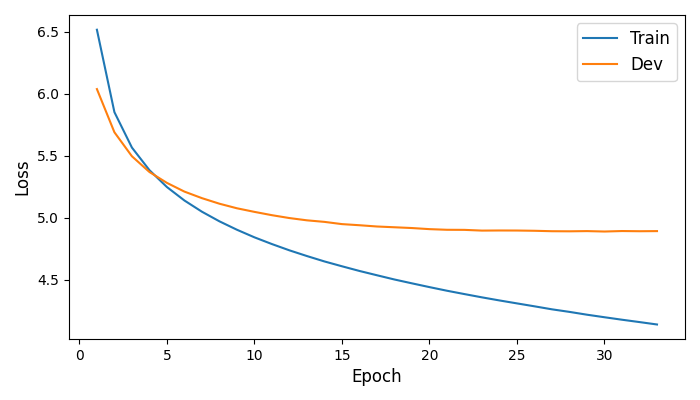
\includegraphics[width=\linewidth]{./images/plot_1_loss.png}
  \caption{Trainig loss for the best model. As we can see, the model starts to overfit very rapidly. The best value for the eval set is reached only after 7 epochs.}
  \label{fig:fig1}
\end{figure}


\bibliographystyle{IEEEtran}

\bibliography{mybib}


\end{document}
